\subsection{Алгоритмы работы системы}
\label{sub:system-design:algorithms}

В общем случае, алгоритм программы представляет собой весь цикл использования программного продукта, начиная с попадания пользователя на начальную страницу и заканчивая получением пользователем желаемых (отчетов, данных).

\textbf{\textit{Алгоритм утверждения запроса на бронирование рабочего места}} является одним из ключевых сценариев в системе управления офисными ресурсами является. Алгоритм реализует бизнес-логику, при которой менеджер, обладающий соответствующими правами, проверяет и одобряет или отклоняет поступивший от сотрудника запрос. После утверждения запроса система резервирует указанное рабочее место за сотрудником, обновляя его статус. Алгоритм проверки и утверждения бронирования содержит в себе несколько этапов проверки правильности входных значений и операций с базой данных.

\begin{enumerate}
    \item \textit{Получение запроса на бронирование}. Из базы данных извлекается объект запроса по его идентификатору. Если запрос помечен как архивный, то дальнейшая обработка запрещается и выполнение завершается с ошибкой. Если запрос помечен как уже обработанный, то выполнение также завершается с ошибкой, так как нет необходимости в повторной обработке запроса. Если тип запроса не является запросом на бронирование рабочего места, то выполнение завершается с ошибкой.
    \item \textit{Проверка пересечений}. В цикле проверяется наличие текущего бронирования данного рабочего места на момент предполагаемой аренды. Если найдено, то выполнение завершается с ошибкой.
    \item \textit{Создание записи бронирования}. Из базы данных извлекается запись сотрудника-заявителя, запись рабочего места, для которого создан обрабатываемый запрос. В базу данных добавляется новая запись бронирования рабочего места, связанная с сотрудником и содержащая данные запроса.
    \item \textit{Обновление запроса на бронирование}. Статус запроса обновляется как успешно обработанный. Сохраняются данные сотрудника, утвердившего запрос на бронирование.
    \item \textit{Обновление статуса рабочего места} происходит в момент наступления времени начала бронирования. Если запрос является запросом на постоянное бронирование рабочего места, обновление статуса происходит немедленно.
    \item \textit{Завершение}. Все действия завершены успешно, бронирование подтверждено.
\end{enumerate}

Схема алгоритма утверждения запроса на бронирование рабочего места представлена на рис.~\ref{fig:system-design:algorithms:approve-workspace-request}.

\begin{figure}
\centering
    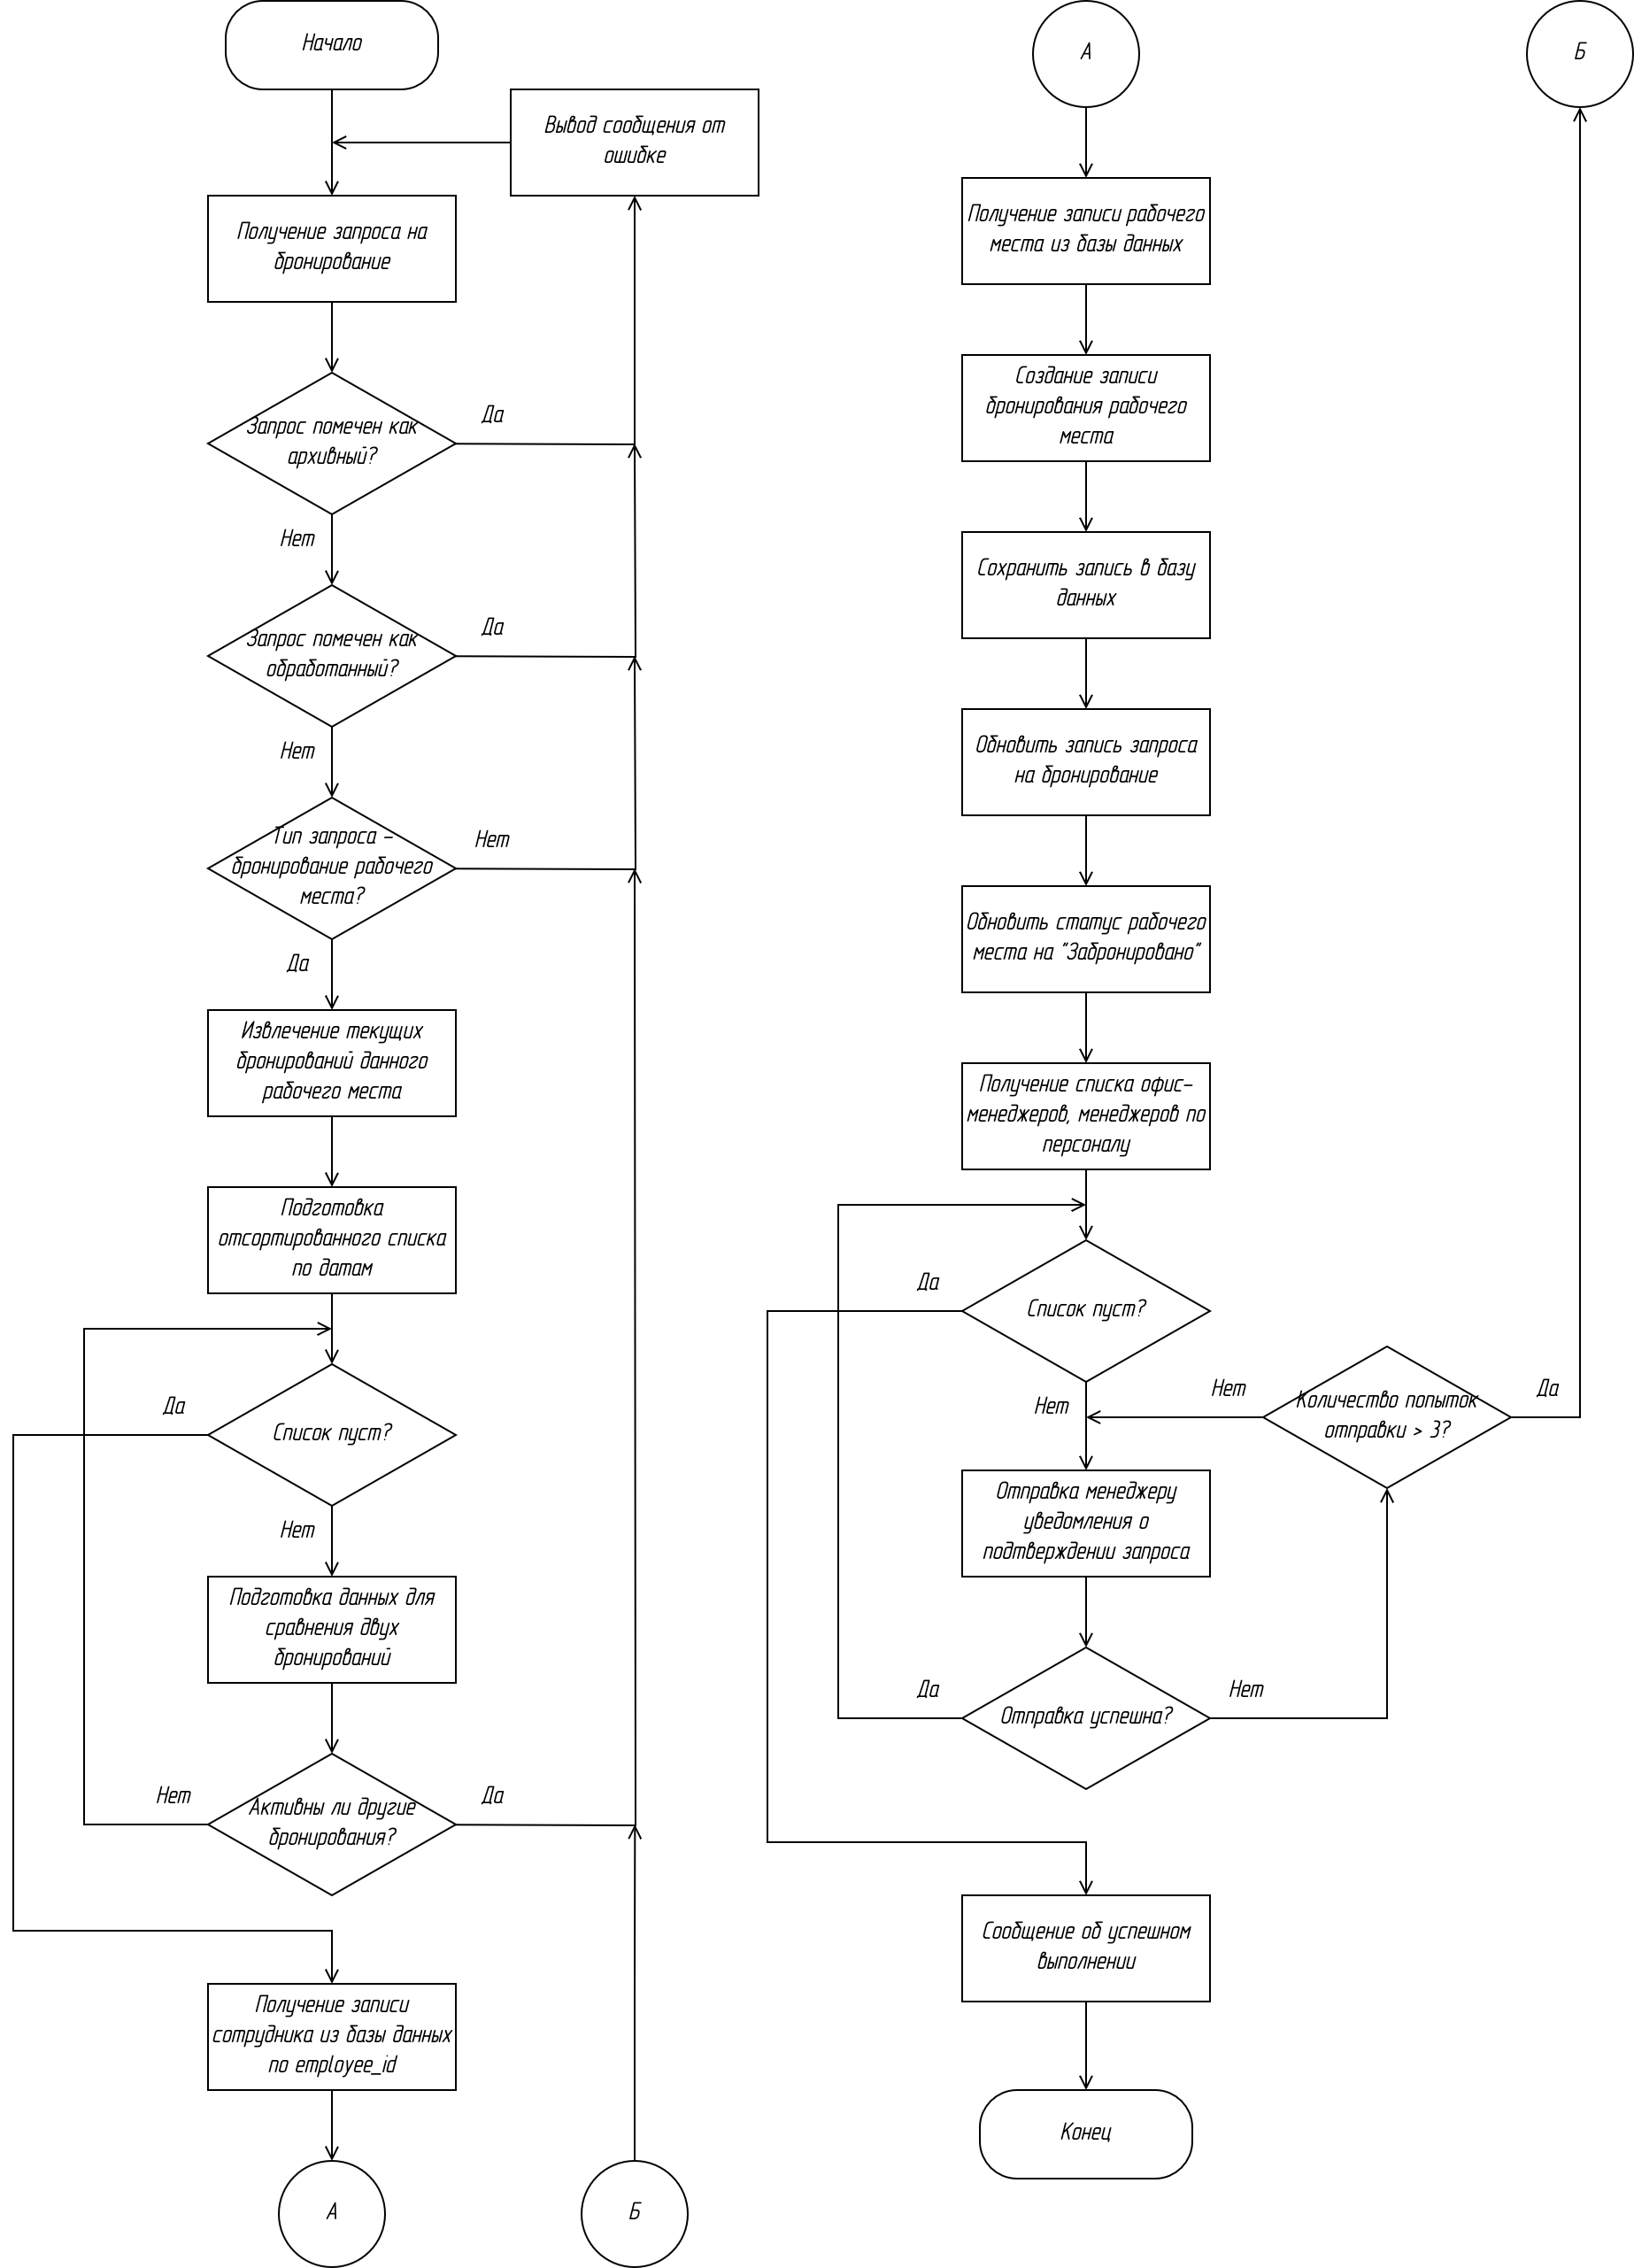
\includegraphics[width=0.99\linewidth]{assets/algorithm-approve-request.png}
    \caption{Схема алгоритма утверждения запроса на бронирование рабочего места}
    \label{fig:system-design:algorithms:approve-workspace-request}
\end{figure}

\textbf{Алгоритм автоматической рассадки сотрудников} предназначен для распределения сотрудников по рабочим местам в офисе на основе заранее заданных параметров. Основная цель~-- оптимально использовать офисные ресурсы, учитывать предпочтения сотрудников и ограничения, связанные с доступностью ресурсов, а также минимизировать ручной труд со стороны менеджеров.

Исходными данными к алгоритму будет являться список сотрудников, нуждающихся в рассадке на определённый период (например, дата или диапазон дат), список доступных рабочих мест, параметры предпочтений сотрудников, данные о занятости рабочих мест (бронирования, текущие рассадки, ремонт/неисправность и т.д.), правила рассадки (заданные компанией, например: сотрудники одного отдела~-- рядом, руководитель~-- возле окна и т.п.). Алгоритм содержит в себе несколько этапов проверки правильности входных значений и операций с базой данных.

\begin{enumerate}
    \item \textit{Получение списка сотрудников}, которые нуждаются в рассадке на определённую дату. В выборку включаются только активные сотрудники, у которых отсутствует назначенное рабочее место на этот день. Исключаются лица, находящиеся в отпуске, командировке, заблокированные или работающие удалённо.
    \item \textit{Определение доступных рабочих мест} путем извлечения из базы данных перечня рабочих мест, которые свободны в указанный период. При этом учитываются следующие ограничения:
    \begin{itemize}
        \item статус рабочего места (только «свободно»);
        \item отсутствие активных бронирований на соответствующий интервал;
        \item исправное техническое состояние;
        \item доступность в рамках политики доступа сотрудника (например, этаж, зона).
    \end{itemize}
    \item \textit{Построение матрицы предпочтений}. Для каждого сотрудника создаётся индивидуальный список предпочтительных рабочих мест, отсортированный по убыванию рейтинга соответствия. Рейтинг формируется на основе множества факторов:
    \begin{itemize}
        \item 3 балла~-- если место соответствует предпочтению «рядом с окном»;
        \item 2 балла~-- если этаж совпадает с желаемым;
        \item 2 балла~-- если место находится в тихой зоне, а сотрудник указал «тишина»;
        \item 2 балла~-- если рядом размещены коллеги из того же отдела;
        \item 1 балл~-- если место расположено вблизи полезной инфраструктуры (принтер, кухня, переговорная);
        \item 0 баллов~-- если критерий не соответствует или отсутствует.
    \end{itemize}
    Для каждого сотрудника инициализируется пустой список предпочтений, производится цикл по всем доступным рабочим местам, где вычисляется рейтинг для каждого места, вследствие чего формируется упорядоченный список подходящих мест. Данные сохраняются в общую матрицу предпочтений сотрудников.
    \item \textit{Проверка достаточности ресурсов}. Перед началом назначения производится проверка: достаточно ли свободных мест для всех сотрудников. Если количество сотрудников превышает число доступных мест, выполняется приоритизация (например, по должности или по срочности присутствия в офисе). Только первые \textit{N} сотрудников получают место, остальные же помечаются как «не рассажены» с соответствующей записью в журнале действий.
    \item \textit{Распределение сотрудников по местам}. Алгоритм последовательно обрабатывает каждого сотрудника, путем выполнения попыток назначить первое доступное место из списка предпочтений. При назначении создаётся запись рассадки, статус рабочего места меняется на «занято». Если ни одно из мест недоступно, сотрудник помечается как «нерассаженный» с указанием причины.
    \item \textit{Формирование отчёта}. По завершении рассадки система формирует отчёт, содержащий фамилию и имя сотрудника, назначенное рабочее место (офис, этаж, номер), степень соответствия предпочтениям, причину отсутствия места (если применимо). Отчёт сохраняется в виде внутреннего документа и может быть передан менеджеру или администратору для дальнейшего анализа.
    \item \textit{Уведомление участников}. На последнем этапе каждому сотруднику отправляется уведомление. В случае, если место назначено~-- сообщение с указанием конкретного места. Если рассадка не произведена~-- отправляется уведомление о необходимости обратиться к менеджеру. Уведомления могут доставляться через email, внутреннюю систему оповещений, или интеграцию с корпоративными мессенджерами.
\end{enumerate}

Результатом выполнения является достижение желаемого результата рассадки сотрудников, при котором каждому сотруднику назначено уникальное рабочее место с учетом предпочтений и ограничений, а также обновление статусов рабочих мест и создание записей о бронировании (рассадке). Алгоритм исключает конфликтные назначения, повышает прозрачность логики рассадки, обеспечивает контроль менеджеров и предоставляет полноценную отчётность по принятым решениям.

Схема алгоритма автоматической рассадки сотрудников представлена на рис.~\ref{fig:system-design:algorithms:automatic-workspace-occupation}.

\begin{figure}
\centering
    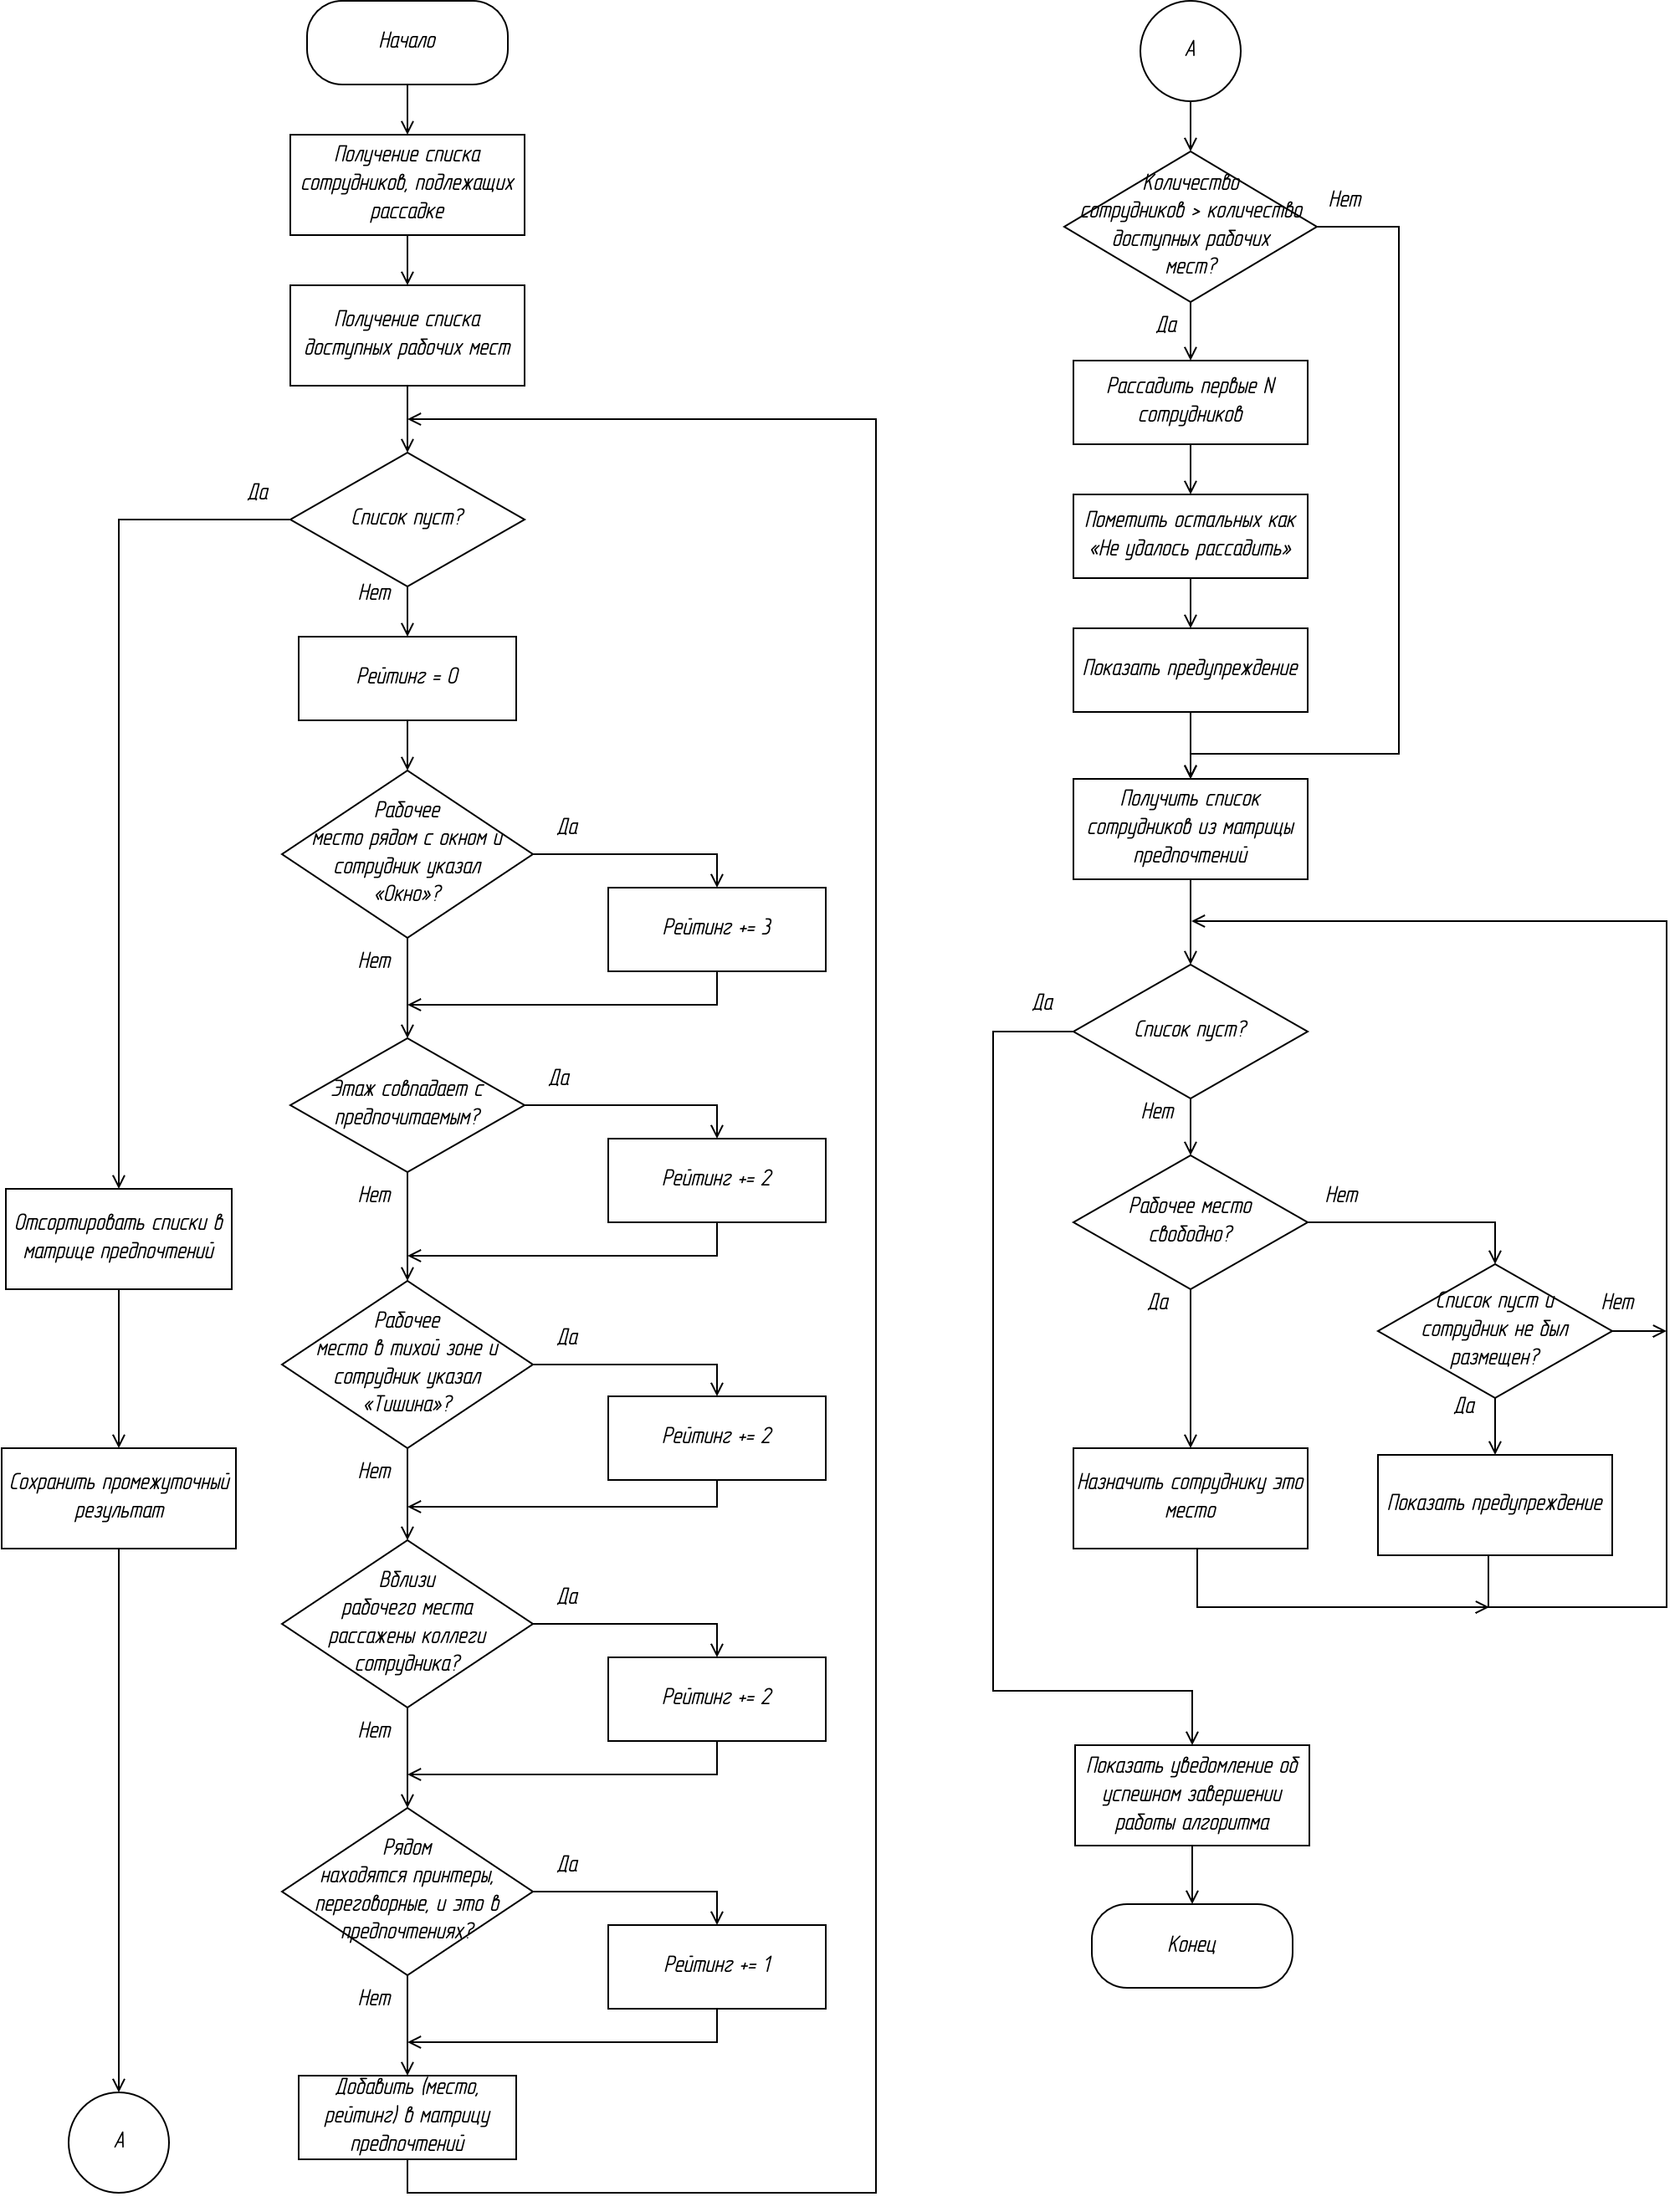
\includegraphics[width=0.99\linewidth]{assets/algorithm-automatic-workspace-occupation.png}
    \caption{Схема алгоритма автоматической рассадки сотрудников}
    \label{fig:system-design:algorithms:automatic-workspace-occupation}
\end{figure}
